\chapter{Implementação}
\label{cap5}



Este capítulo descreve a implememtação dos micorsserviços que compõe o jogo em cada arquitetura.
%
Isto é necessário pois as escolhas técnicas, envolvendo as linguagens adotadas, as tecnologias utilizadas e as boas práticas aplicadas no desenvolvimento das aplicações, interferem na qualidade (consumo de recursos e o desempenho das aplicações) dos microsserviços.


Devido às diversas possibilidades de linguagens de programação e bibliotecas disponíveis, a Seção~\ref{sec:tecnologias} tem o objetivo de descrever as tecnologias utilizadas para o desenvolvimento das aplicações e justificar tais escolhas.
%
Além disso, a Seção~\ref{sec:tecnologias} apresenta o conjunto de serviços externos utilizados para facilitar o desenvolvimento dos microsserviços.
%
Os serviços externos, apesar de não estarem diretamente implementados na arquitetura das soluções, foram utilizados durante o processo e por tal motivo devem ser evidenciados.



Diante da complexidade das arquiteturas de microsserviços desenvolvidos, torna-se necessário descrever quais microsserviços foram implementados, e como estão dispostos na rede.
%
Para este fim, a Seção~\ref{sec:interconexao} contextualiza a interconexão dos microsserviços desenvolvidos.



\section{Tecnologias Utilizadas}
\label{sec:tecnologias}



A seleção das tecnologias e bibliotecas que são executadas nas aplicações é importante, visto que estas implicam diretamente no desempenho e consumo de recursos das arquiteturas selecionadas.
%
Entretanto, essa seleção precisa estar de acordo com as regras de negócio impostas para os testes.



Inicialmente, existe uma preocupação com a linguagem de programação utilizada, visto que esta precisa ter um bom desempenho, um suporte a programação paralela e, ao mesmo tempo, conter bibliotecas que auxiliem no desenvolvimento ágil dos serviços.
%
Neste sentido, foi levantado um conjunto de linguagens de programação, o qual viabiliza o projeto de acordo com os seguintes critérios:



\begin{itemize}
  \item Alto desempenho para programas paralelos;
  \item Biblioteca para conexão com banco de dados PostgreSQL;
  \item Biblioteca para uso de cache (Redis);
  \item Biblioteca para escrita de serviços \ac{rpc}, sobre o protocolo \ac{tcp};
  \item Biblioteca para escrita de serviços \textit{web}, com \ac{api} no formato \ac{json};
  \item Linguagem compilada;
  \item Linguagem com tipagem estática; e
  \item Simplicidade de escrita de código, preferencialmente.
\end{itemize}



A partir destes critérios, a linguagem selecionada foi a linguagem GoLang, por se tratar de uma linguagem a qual o autor possui domínio e satisfaz os critérios aqui listados.
%
Outro critério, o qual é implícito para o desenvolvimento, é a homogeneidade da linguagem de programação em todos os microsserviços.
%
Tal necessidade gera o benefício da escrita de código reutilizável, como o núcleo de regras de negócio que pode ser aplicado a todas as arquiteturas desenvolvidas.



Assim, foi selecionada uma única linguagem de programação compatível com a viabilização do projeto.
%
Em função da diversidade de bibliotecas disponíveis, também é necessário definir quais bibliotecas foram utilizadas para o desenvolvimento das arquiteturas dos microsserviços.
%
Dentre as bibliotecas utilizadas, destacam-se:



\begin{itemize}
  \item gin: Servidor Web para serviços de alto desempenho;
  \item gorm: Biblioteca de objetos relacionais, a qual suporta conexão direta ao banco PostgreSQL;
  \item go-redis: Biblioteca para conexão ao serviço Redis;
  \item net/rpc: Biblioteca nativa da linguagem GoLang para escrita de serviços \ac{rpc} sobre o protocolo \ac{tcp};
  \item graphite: Biblioteca de conexão ao banco de métricas; e
  \item testify: Biblioteca auxiliar a suíte nativa de testes da linguagem.
\end{itemize}



Estas bibliotecas foram utilizadas na camada de infraestrutura, sendo seu uso aplicado a todas as arquiteturas.
%
A camada de infraestrutura é responsável pela realização da interação entre a rede e as regras de negócio dos microsserviços.


Destaca-se, dentre as bibliotecas citadas, a biblioteca testify.
%
Tal biblioteca foi utilizada na garantia de integridade das aplicações desenvolvidas.
%
Sua finalidade é realizar a inspeção automatizada do funcionamento da aplicação.
%
Entretanto, a biblioteca não é utilizada durante a execução da aplicação, denotando-se como uma biblioteca auxiliar.



As bibliotecas auxiliares foram utilizadas no processo de integração contínua.
%
O processo de integração contínua foi implantado utilizando os serviços externos Github e TravisCI.
%
Este processo é descrito como processo de construção na arquitetura Willson, sendo responsável pelo teste e envio de imagens de contêineres a um serviço de registro na nuvem.




Após descrever as tecnologias utilizadas, faz-se necessário descrever o ambiente distribuído desenvolvido.
%
Esta descrição é necessária a fim de garantir uma melhor visibilidade dos microsserviços implementados, na qual são citados na análise.



\section{Interconexão entre os microsserviços}
\label{sec:interconexao}



A interconexão entre os microsserviços refere-se ao projeto de rede de uma arquitetura qualquer, disponibilizando visualmente a camada de rede.
%
Ao todo foram implementados onze microsserviços, os quais possuem a comunicação através de troca de mensagens.
%
Tais conexões entre si, com os bancos de dados e com os seus respectivos clientes, foram definidas pelos autores das arquiteturas.
%
Consequentemente, torna-se relevante descrever a interconexão entre os microsserviços, exibindo assim seus protocolos de comunicação de rede:


\begin{itemize}
 \item A arquitetura Rudy contém um microsserviço intermediário para conexão com o banco de dados.
%
Esta disposição de microsserviços está exposta na Subseção~\ref{sec:inter_rudy}.

 \item A arquitetura Salz remove a responsabilidade de mensageria do jogo do microsserviço de jogo.
%
Outra alteração é a exposição do microsserviço de autenticação como uma interface pública na rede, permitindo a conexão a partir dos clientes.
%
Esta disposição de microsserviços da arquitetura Salz é exposta na Subseção~\ref{sec:inter_salz}.

\item A arquitetura Willson tem o funcionamento semelhante a arquitetura Rudy, porém não utiliza um microsserviço intermediário para organização de consultas ao banco de dados.
%
A disposição dos microsserviços nesta arquitetura é visível na Subseção~\ref{sec:inter_willson}.

\end{itemize}

As arquiteturas foram desenvolvidas com escopo limitado.
%
Esta limitação é descrita na Subseção~\ref{sec:SimulaCliente}, no qual evidenciam-se quais ações os clientes realizam no serviço.
%
Tal redução de escopo visa analisar as funcionalidades básicas de um serviço \ac{mmorpg} evitando regras de negócio específicas.



\subsection{Rudy}
\label{sec:inter_rudy}


A arquitetura Rudy foi implementada em versão reduzida para o escopo dos testes.
%
A arquitetura Rudy implementada contém quatro microsserviços e dois banco de dados, sendo um para dados permanentes (PostgreSQL) e um para dados temporários (Redis).
%
Os seus microsserviços estão listados na Tabela~\ref{tab:inter_rudy}.

\begin{table}[htb!]
\centering
\begin{adjustbox}{max width=\textwidth}
\caption{Microsserviços da arquitetura Rudy.}
\label{tab:inter_rudy}
\begin{tabular}{l|l|l}
\hline
Nome            & Protocolo            & Público na Rede \\ \hline
 rgame          & \ac{rpc}/\ac{tcp}    & \checkmark     \\ \hline
 rweb           & \ac{http}/\ac{json}  & \checkmark     \\ \hline
 rauth          & \ac{rpc}/\ac{tcp}    &                \\ \hline
 rcrud          & \ac{rpc}/\ac{tcp}    &                \\ \hline
\end{tabular}
\end{adjustbox}

Fonte: O próprio autor.
\end{table}

A Tabela~\ref{tab:inter_rudy} relaciona os microsserviços aos protocolos na qual respondem e a sua visibilidade, do ponto de vista do cliente.
%
Isto significa que, microsserviços públicos a rede podem e são acessados pelos clientes.
%
Os microsserviços da arquitetura Rudy, descritos na Tabela~\ref{tab:inter_rudy}, possuem funcionalidades próprias.
%
As funcionalidades de cada microsserviço são:



\begin{itemize}
  \item \textit{rgame}: Gerencia o posicionamento dos personagens, a execução das operações do mundo e a troca de mensagens do \textit{chat} do jogo. Ele também é responsável por autenticar contas ao mundo do jogo.
  \item \textit{rweb}: Recebe requisições web como uma \ac{api}, essas requisições podem ser referentes a criação de novas contas ou personagens para o jogo.
  \item \textit{rauth}: Autentica e garante uma única conexão por conta em determinada arquitetura.
  \item \textit{rcrud}: Realiza o acesso ao banco de dados, retornando os dados da consulta a qual é requisitada.
\end{itemize}



Dado tais características, temos um ponto de atenção no microsserviço \textit{rcrud}, o qual cria uma camada de acesso ao banco de dados.
%
Este padrão de projeto tende a facilitar a manutenção do banco de dados, centralizando todas as operações a dados temporários e permanentes.

O objetivo do microsserviço ~\textit{rcrud} é mover o escopo de consulta a dados em um ponto centralizado, evitando assim falhas ao armazenar e obter tais dados.
%
Este processo é escalável, entretanto adiciona uma camada maior ao obter os dados, na qual tende a aumentar o tempo de resposta para as operações ao banco.
%
A disposição da arquitetura Rudy está visível na Figura~\ref{fig:interconexao_rudy}.



\begin{figure}[htb!]
  \caption{Interconexões da arquitetura Rudy.}
  \label{fig:interconexao_rudy}
  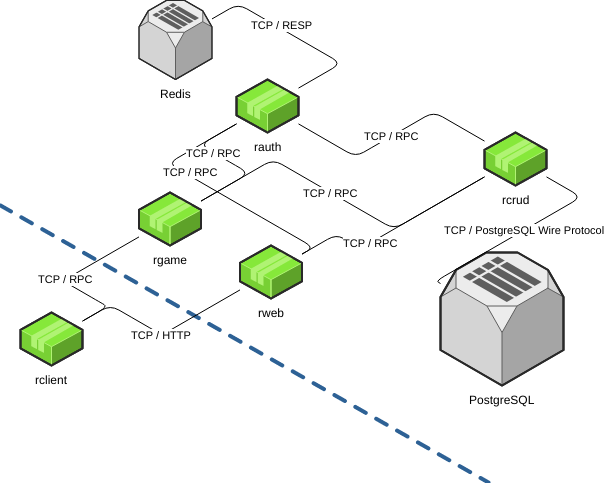
\includegraphics[width=0.8\textwidth]{figuras/interconexoes/rudy.png}
  \centering

  Fonte: O próprio autor.
\end{figure}

Outro ponto de atenção é o acesso ao microsserviço de autenticação \textit{rauth}, o qual pode ser visualizado na Figura~\ref{fig:interconexao_rudy}.
%
Tal microsserviço é privado, dessa forma o microsserviço de mundo fica responsável por ser um ponto intermediário de comunicação entre o cliente e o serviço que realiza a autenticação.
%
Este padrão de projeto é comum em aplicações Web, entretanto não recomendado pelo padrão sugerido  \ac{jwt}.

%
Mesmo não sendo um padrão recomendado, tal característica não deve ter um impacto significativo para arquiteturas de jogos \ac{mmorpg}, visto que esta operação é realizada poucas vezes no serviço.
%
O padrão \ac{jwt} recomenda tornar o microsserviço de autenticação público, na qual o cliente realiza a autenticação diretamente com o microsserviço de autenticação, reduzindo o tráfego interno de rede.


%Entretanto, a arquitetura Salz realiza alterações compatíveis com o padrão \ac{jwt} e remove microsserviços privados, usando uma interconexão de microsserviços plana.
%
%Dessa forma, torna-se interessante descrever tais características a fim de permitir comparações na arquitetura.



\subsection{Salz}
\label{sec:inter_salz}



A arquitetura Salz, em versão reduzida para o escopo dos testes, contém quatro microsserviços e dois bancos de dados, sendo um para dados permanentes (PostgreSQL) e um para dados temporários (Redis).
%
Os seus microsserviços estão listados na Tabela~\ref{tab:inter_salz}.



\begin{table}[htb!]
\centering
\begin{adjustbox}{max width=\textwidth}
\caption{Microsserviços da arquitetura Salz.}
\label{tab:inter_salz}
\begin{tabular}{l|l|l}
\hline
Nome            & Protocolo            & Público na Rede \\ \hline
 sgame          & \ac{rpc}/\ac{tcp}    & \checkmark     \\ \hline
 schat          & \ac{rpc}/\ac{tcp}    & \checkmark     \\ \hline
 sweb           & \ac{http}/\ac{json}  & \checkmark     \\ \hline
 sauth          & \ac{rpc}/\ac{tcp}    & \checkmark     \\ \hline
\end{tabular}
\end{adjustbox}

Fonte: O próprio autor.
\end{table}



Os microsserviços da arquitetura Salz, descritos na Tabela~\ref{tab:inter_salz}, possuem funcionalidades próprias.
%
A funcionalidade de cada microsserviço é:



\begin{itemize}
  \item \textit{sgame}: Gerencia o posicionamento dos personagens, execução das operações do mundo e troca de mensagens do chat do jogo.
  \item \textit{schat}: Gerencia mensagens entre jogadores e possui um forte acoplamento com o microsserviço \textit{sgame}.
  \item \textit{sweb}: Recebe requisições web como uma \ac{api} a fim de criar novas contas e novos personagens para o jogo.
  \item \textit{sauth}: Autentica e garante uma única conexão por conta em determinada arquitetura.
\end{itemize}



Ao definir as funcionalidades dos microsserviços da arquitetura Salz, nota-se que o microsserviço \textit{schat} possui algumas particularidades.
%
Tal microsserviço é responsável por gerenciar todo o serviço de chat da arquitetura, seja baseado em região de interesse ou global.
%
Entretanto, a informação de posicionamento não está armazenada neste microsserviço.
%
Nesse sentido, esta característica necessita de uma sincronização de dados, a qual implica diretamente em custo de recurso ou tempo de resposta para o cliente.
%
A topologia de rede da arquitetura Salz pode ser visualizada na Figura~\ref{fig:interconexao_salz}.



\begin{figure}[htb!]
  \caption{Interconexões da arquitetura Salz.}
  \label{fig:interconexao_salz}
  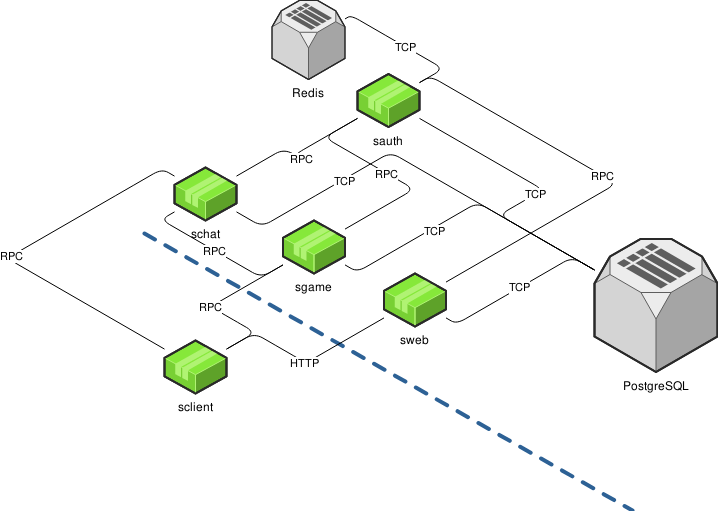
\includegraphics[width=0.8\textwidth]{figuras/interconexoes/salz.png}
  \centering

  Fonte: O próprio autor.
\end{figure}



Outra característica desta arquitetura é a comunicação direta entre o microsserviço de autenticação \textit{sauth} e o cliente.
%
Isto evita uma conexão intermediária, a qual utilizaria o microsserviço \textit{sgame}.
%
A comunicação direta realizada permite que exista uma maior vazão de dados sobre autenticação e sessão.
%
Outro ponto a ser ressaltado é a possibilidade de utilizar \ac{jwt} para autenticação, sem a necessidade de verificação pelo próprio microsserviço de autenticação.



Com a interconexão da arquitetura Salz sendo feita de forma direta, o sistema de autenticação torna-se independente, permitindo assim adicionar novos serviços de forma flexível.
%
Também nota-se uma possível utilização de verificação de sessão por assinatura digital.
%
Essa assinatura digital é utilizada no microsserviço de autenticação, diminuindo o consumo da rede para mensagens de verificação pelo serviço de autenticação.
%
Entretanto, não foi utilizado tal método de validação de sessão.




O método de autenticação atual consiste na validação de assinatura utilizando o banco de dados de dados temporários (\textit{cache}).
%
Esse método utiliza uma comunicação entre os microsserviços \textit{schat} e \textit{sgame} com o microsserviço \textit{sauth}.
%
Esta escolha foi realizada para manter os mesmos métodos de autenticação em todas as arquiteturas, evitando variação de algoritmo ou tecnologia.



Definidas as características da arquitetura Salz, a sincronização de posições entre o microsserviço \textit{schat} e \textit{sgame} pode ser um ponto de atenção, logo deve-se atentar a frequência da sincronização necessária pela regra de negócio do jogo implementado.
%
%Dessa forma, a arquitetura Willson propõe um ponto intermediário entre as arquiteturas Salz e Rudy, tornando-se interessante descrever suas alterações.



\subsection{Willson}
\label{sec:inter_willson}


A arquitetura Willson, em versão reduzida para o escopo dos testes, contém três microsserviços e dois bancos de dados.
%
Os microsserviços de banco de dados são um para dados permanentes (PostgreSQL) e um para dados temporários (Redis).
%
Os microsserviços da arquitetura Willson estão listados na Tabela~\ref{tab:inter_willson}.



\begin{table}[htb!]
\centering
\begin{adjustbox}{max width=\textwidth}
\caption{Microsserviços da arquitetura Willson.}
\label{tab:inter_willson}
\begin{tabular}{l|l|l}
\hline
Nome            & Protocolo            & Público na Rede \\ \hline
 wweb           & \ac{http}/\ac{json}  & \checkmark     \\ \hline
 wgame          & \ac{rpc}/\ac{tcp}    & \checkmark     \\ \hline
 wauth          & \ac{rpc}/\ac{tcp}    &                \\ \hline
\end{tabular}
\end{adjustbox}

Fonte: O próprio autor.
\end{table}


Os microsserviços da arquitetura Willson, descritos na Tabela~\ref{tab:inter_willson}, possuem funcionalidades próprias.
%
As funcionalidades de cada microsserviço são:



\begin{itemize}
  \item \textit{wgame}: Gerencia o posicionamento dos personagens, a execução das operações do mundo e a troca de mensagens do chat do jogo e também gerencia a sessão do jogador, que têm um forte acoplamento com o microsserviço \textit{wauth}.
  \item \textit{wweb}: Recebe requisições web como uma \ac{api} a fim de criar novas contas e novos personagens para o jogo.
  \item \textit{wauth}: Autentica e garante uma única conexão por conta em determinada arquitetura.
\end{itemize}



Definidos os microsserviços da arquitetura Willson, na Tabela~\ref{tab:inter_willson}, uma característica interessante é a ausência de um microsserviço de gerência de mensagens de \textit{chat} e um intermediário para gestão de dados do banco.
%
Estas características tornam a arquitetura mais simples, dividindo os microsserviços em domínios específicos, os quais têm foco em escalabilidade.
%
A interconexão da arquitetura Willson pode ser visualizada na Figura~\ref{fig:interconexao_willson}.



\begin{figure}[htb!]
  \caption{Interconexões da arquitetura Willson.}
  \label{fig:interconexao_willson}
  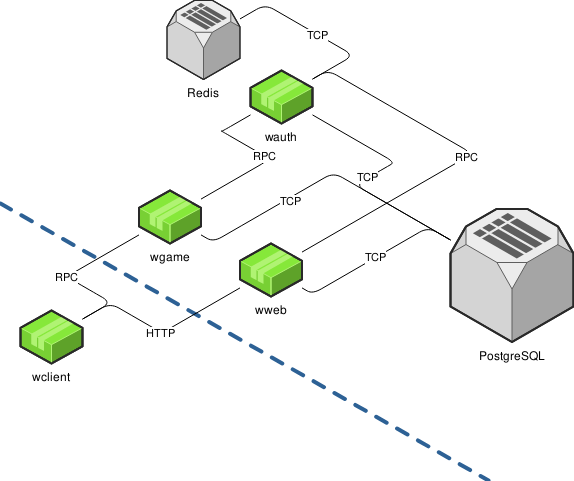
\includegraphics[width=0.8\textwidth]{figuras/interconexoes/willson.png}
  \centering

  Fonte: O próprio autor.
\end{figure}



A Arquitetura Willson, conforme visualizado na Figura~\ref{fig:interconexao_willson}, simplifica a interconexão dos microsserviços e reduz um microsserviço de sua topologia.
%
Dessa forma, espera-se que ocorra uma diminuição no consumo de rede e no tempo de resposta quando comparado as demais arquiteturas.



\section{Ambiente de Testes}
\label{sec:ambiente_de_testes}



O ambiente de testes refere-se ao ambiente físico ou virtual a qual as arquiteturas e clientes foram implantados.
%
Este ponto é importante para permitir a reprodução dos experimentos executados.



Em um cenário de jogos massivos, encontram-se duas regiões distintas.
%
Em uma visão superficial, estas regiões provém do paradigma Cliente-Servidor, como visível na Figura~\ref{fig:cenario_cliente_servidor}.

\begin{figure}[htb!]
  \caption{Cenário Cliente Servidor Genérico.}
  \label{fig:cenario_cliente_servidor}
  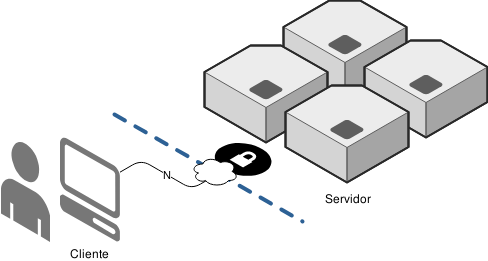
\includegraphics[width=0.8\textwidth]{figuras/ambiente/cs.png}
  \centering

  Fonte: O próprio autor.
\end{figure}



A Figura~\ref{fig:cenario_cliente_servidor} exibe um usuário que utiliza um cliente genérico para conectar em um servidor genérico.
%
Este servidor pode ser uma ou mais máquinas físicas ou virtuais, utilizando múltiplos processos.
%
Em específico, para jogos \ac{mmorpg}, o cliente estará em uma rede diferente do servidor, visto que o objetivo do jogo é prover um mundo compartilhado.



A rede utilizada pelo cliente usualmente é uma rede \ac{lan}, a qual conecta-se pela Internet na rede do servidor.
%
Para os testes, tal rede possui características específicas para gerenciar a implantação dos clientes de forma automatizada, a qual será abordado na Subseção~\ref{sec:net_cliente}.




Neste contexto, há duas redes que separam os ambientes de microsserviços e serviços satélites destas aplicações.
%
Esta separação física é necessária nos testes para adicionar um limitador de transporte de dados e latência, tal qual ocorre em aplicações que executam em produção para a categoria de jogos \ac{mmorpg}.
%
Esta separação é visível na Figura~\ref{fig:net_completa}.

\begin{figure}[htb!]
  \caption{Cenário Cliente Servidor Genérico.}
  \label{fig:net_completa}
  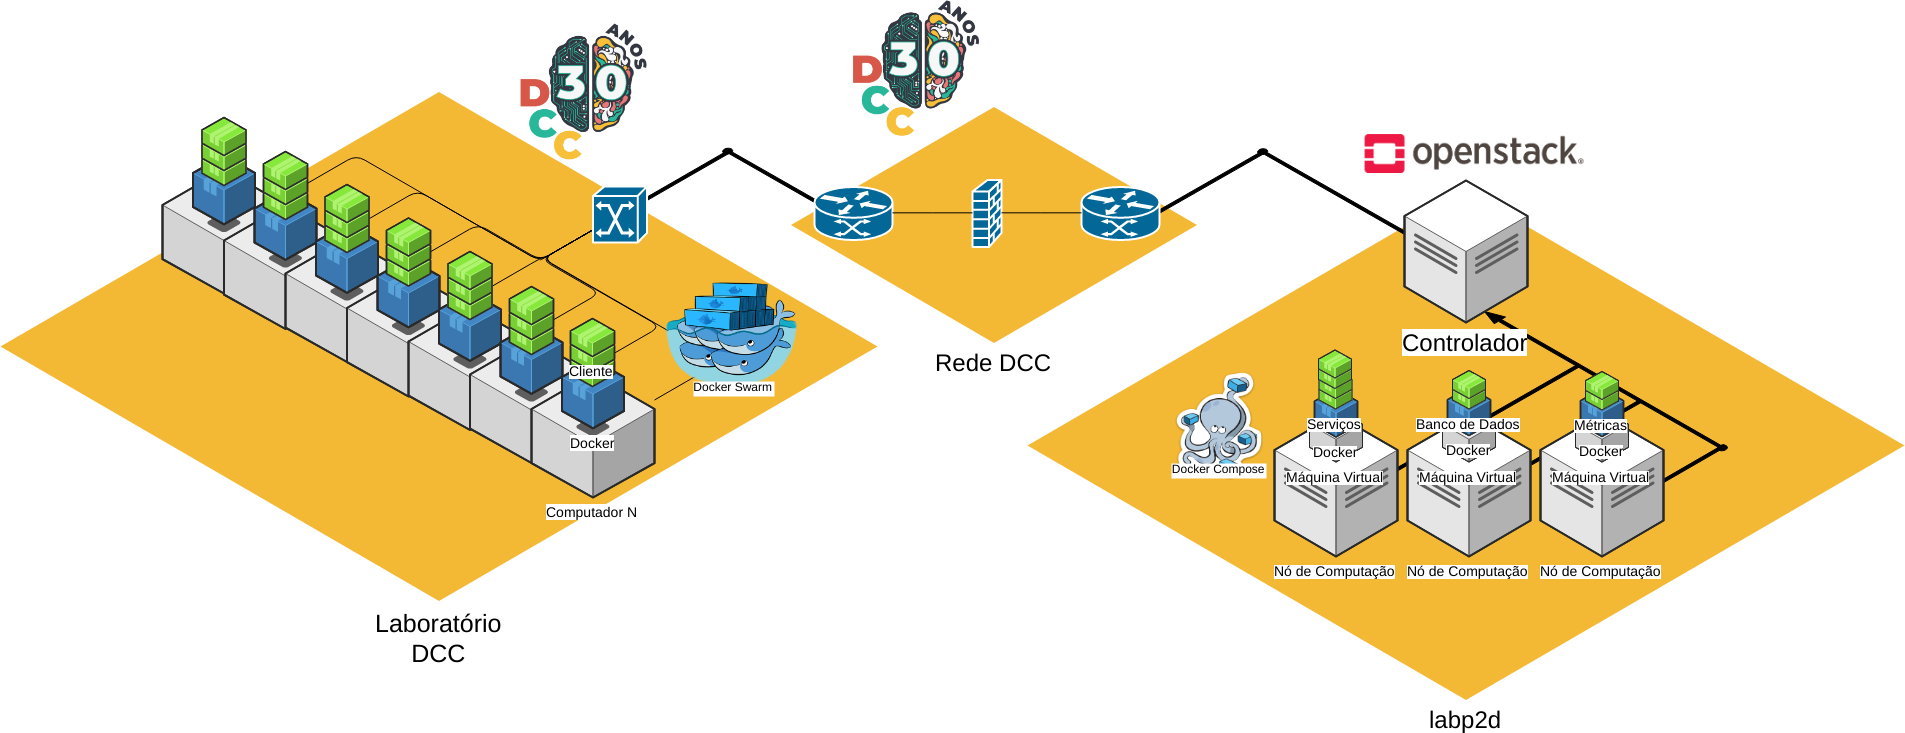
\includegraphics[width=\textwidth]{figuras/ambiente/full.png}
  \centering

  Fonte: O próprio autor.
\end{figure}

As redes do cliente e servidor, visíveis na Figura~\ref{fig:net_completa}, são implantadas em plataformas diferentes.
%
Os dados técnicos de cada rede são descritos nas Subseções~\ref{sec:net_server} e~\ref{sec:net_cliente}.



Nota-se que existe uma rede intermediária desempenhando o papel da separação física entre servidor e cliente.
%
No atual trabalho esta rede pertence ao \ac{dcc}.

\subsection{Rede do Servidor}
\label{sec:net_server}



A rede do servidor é implantada sobre uma infraestrutura virtualizada, gerenciada pelo OpenStack na versão \textit{Rocky}.
%
Tal estrutura garante um ambiente próximo ao utilizado em produção para serviços \ac{mmorpg}.


Entretanto, como exibido na Seção~\ref{sec:interconexao}, os serviços para jogos \ac{mmorpg} são compostos por múltiplos processos implementando uma arquitetura de microsserviços.
%
Por este motivo, torna-se interessante dividir o ambiente do servidor em sub-redes.
%
Esta divisão pode ser visualizada na Figura~\ref{fig:network_server}



\begin{figure}[htb!]
  \caption{Sub-redes do servidor}
  \label{fig:network_server}
  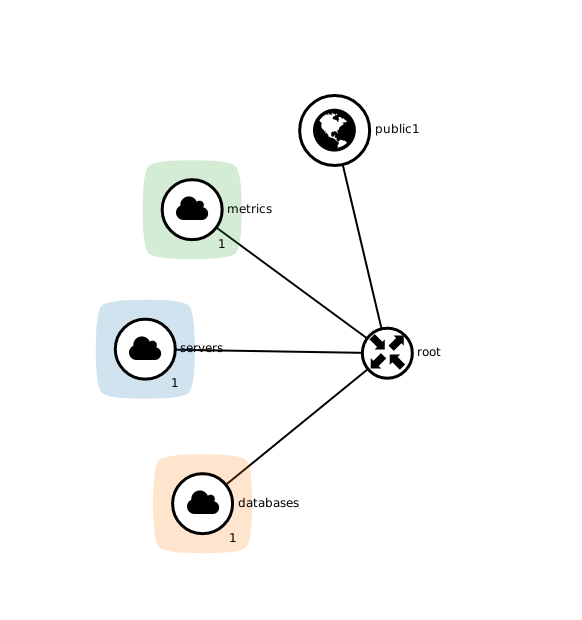
\includegraphics[width=0.8\textwidth]{figuras/network/circles_only_networks.png}
  \centering

  Fonte: O próprio autor.
\end{figure}



Como exibido na Figura~\ref{fig:network_server}, para o contexto deste trabalho, faz sentido dividir em sub-redes para os seguintes contextos:



\begin{itemize}
  \item Microsserviços: Contém os processos das arquiteturas Rudy, Salz e Willson;
  \item Banco de Dados: Contém os processos de banco de dados permanente e temporário; e
  \item Métricas: Contém serviços para armazenamento de dados em ordem temporal.
\end{itemize}



Esta divisão garante o isolamento apropriado para gerenciamento dos projetos na rede, facilitando a implantação dos microsserviços.
%
Sua realização ocorreu utilizando sub redes no sistema OpenStack, no qual é definido como um sistema de gerenciamento de unidades de computação, armazenamento e comunicação sobre um aglomerado computacional~\cite{open_stack_bib}.
%
O escopo geral do OpenStack é visualizado na Figura~\ref{fig:arch_open_stack}.



\begin{figure}[htb!]
  \caption{Arquitetura abstraída do OpenStack}
  \label{fig:arch_open_stack}
  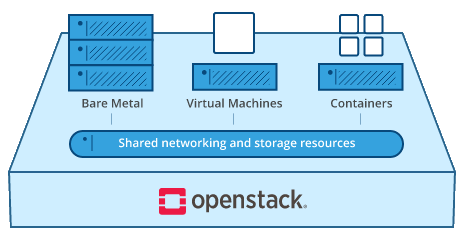
\includegraphics[width=0.8\textwidth]{figuras/ambiente/openstack.png}
  \centering

  Fonte: ~\cite{open_stack_bib}.
\end{figure}



Como visualizado na Figura~\ref{fig:arch_open_stack}, o ambiente virtual é gerado sobre máquinas servidoras, nas quais são gerenciadas pelo OpenStack.
%
O ambiente virtual pode conter serviços, como por exemplo bancos de dados, armazenamento de arquivos, máquinas virtuais ou contêineres~\cite{open_stack_bib}.



Entretanto, no contexto dos testes, faz sentido utilizar máquinas virtuais de tal forma que pode-se executar \textit{scripts} para acessar dados da máquina virtual e métricas do gestor de contêineres.
%
Desta forma, torna-se independente do ambiente físico real que está executando as aplicações.



Conforme a escolha de execução do servidor sobre máquinas virtuais, surge a necessidade da configuração de sub-redes no ambiente do servidor.
%
Certamente é possível construir um ambiente com uma única sub-rede realizando esta divisão por redes do gestor de contêineres, porém tal escolha não é uma boa prática para organização do projeto, visto que existem partes do serviço que possuem contextos diferentes.
%
Deste modo, foram criadas sub-redes de acordo com os contextos levantados na Figura~\ref{fig:network_server}.
%
A Tabela~\ref{tab:subredes} mostra a divisão de tais subredes, conforme a faixa de \ac{ip} aplicada.



\begin{table}[htb!]
\centering
\begin{adjustbox}{max width=\textwidth}
\caption{Subredes da rede do servidor.}
\label{tab:subredes}
\begin{tabular}{|l|l|}
\hline
Nome da subrede & Faixa          \\ \hline
metrics         & 192.168.0.0/24 \\ \hline
databases       & 192.168.1.0/24 \\ \hline
servers         & 192.168.2.0/24 \\ \hline
\end{tabular}
\end{adjustbox}

Fonte: O próprio autor.
\end{table}



As subredes, descritas na Tabela~\ref{tab:subredes}, foram criadas seguindo um padrão de faixa de \ac{ip} conforme a configuração exigida pela nuvem Tchê.
%
As faixas de \ac{ip} dependem das redes externas a nuvem computacional gerenciada pelo OpenStack.
%
Entretanto, tal configuração não implica na performance da aplicação, somente em sua organização.

Cada subrede possui uma máquina virtual para execução dos serviços.
%
O esquema das máquinas virtuais está visível na Figura~\ref{fig:virtual_machines}.




\begin{figure}[htb!]
  \caption{Sub-redes do servidor com as máquinas virtuais}
  \label{fig:virtual_machines}
  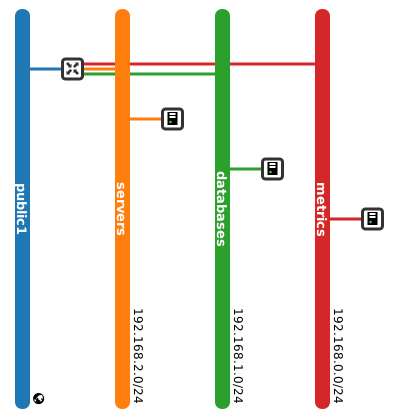
\includegraphics[width=0.5\textwidth]{figuras/network/bars.png}
  \centering

  Fonte: O próprio autor.
\end{figure}



Conforme visível na Figura~\ref{fig:virtual_machines}, cada sub-rede possui uma única máquina virtual, sendo que esta executará um gerenciador de contêineres com os serviços necessários para a execução do servidor.
%
As máquinas virtuais por sua vez possuem configurações distintas e essas configurações são exibidas na Tabela~\ref{tab:configuracao_das_maquinas}.



\begin{table}[htb!]
\centering
\begin{adjustbox}{max width=\textwidth}
\caption{Configurações das máquinas virtuais do servidor.}
\label{tab:configuracao_das_maquinas}
\begin{tabular}{|l|l|l|l|l|l|}
\hline
Nome              & Sistema Operacional            & IP          & vCPU    & Memória & Armazenamento \\ \hline
server\_machine   & Ubuntu LTS 18.04 Bionic Beaver & 192.168.2.* & 4 Cores & 8 GB    & 40GB          \\ \hline
database\_machine & Ubuntu LTS 18.04 Bionic Beaver & 192.168.1.* & 4 Cores & 8 GB    & 40GB          \\ \hline
metric\_machine   & Ubuntu LTS 18.04 Bionic Beaver & 192.168.0.* & 4 Cores & 8 GB    & 120GB         \\ \hline
\end{tabular}
\end{adjustbox}

Fonte: O próprio autor.
\end{table}



Conforme exibido na Tabela~\ref{tab:configuracao_das_maquinas}, a única variação entre as configurações das máquinasa virtuais do servidor é o armazenamento da máquina virtual \textit{metric\_machine}.
%
Tal característica é dada pela necessidade de armazenamento de métricas, nas quais precisam de volumes de dados dedicados a este serviço.



Em todas as sub-redes, por padrão, foi utilizado o gestor de contêineres Docker Compose.
%
Este gestor de contêineres permite executar aplicações de multi-contêineres usando como entrada um arquivo \ac{yaml}.
%
Este formato é específico para notação de dados legíveis a humanos.



Entretanto, a rede do cliente interfere diretamente na execução dos experimentos, visto que possui características próprias.
%
Nesse sentido, torna-se necessário a descrição da rede do cliente.

\subsection{Rede do Cliente}
\label{sec:net_cliente}


Os clientes executaram sobre uma rede \ac{lan}.
%
Estes computadores formam um aglomerado de contêineres para realizar o acesso as arquiteturas na rede do servidor (Subseção~\ref{sec:net_server}).
%
Os computadores utilizados possuem características próprias, as quais devem ser citadas para melhor compreendimento das características da rede de clientes.

O aglomerado computacional é composto por nove computadores.
%
Todos os computadores possuem 8 \textit{cores}, 16 GB de memória e 1TB de armazenamento.

Em especial, percebe-se que este aglomerado é composto por características homogênias.
%
Este ambiente foi montado com tais características para remover complexidade, evitando possíveis problemas de diferença de sistema operacional ou hardware.

Para formar o aglomerado de contêineres foi utilizado a tecnologia \textit{Docker Swarm}.
%
Tal tecnologia permite o controle da infraestrutura pelo \textit{Docker Engine} (Serviço de controle de contêineres) de forma remota, podendo-se definir os serviços em arquivos \ac{yaml}, a partir das máquinas administradoras do aglomerado.

Outra característica importante do \textit{Docker Swarm} é que, pelo fato de ser uma interface de gerenciamento do \textit{Docker Engine}, podemos obter dados de consumo de recursos individuais por contêinerer.
%
Nesse sentido, permite-se obter os recursos consumidos por contêinerer registrado no serviço Docker.

Seguindo o padrão de testes, definido na Subseção~\ref{sec:cap4_testes}, foi executado o seguinte protocolo de testes:

\begin{enumerate}
  \item Executar 3 vezes as arquiteturas com zero jogadores simultâneos, por 5 minutos;
  \item Executar 3 vezes as arquiteturas com um jogador apenas; e
  \item Executar 3 vezes as arquiteturas com zero jogadores simultâneos, aumentando a cada 30 segundos o número jogadores (um por vez) ao serviço, até o serviço obter algum erro interno de microsserviço e terminar a sua execução por erro interno ou chegar a 100 jogadores simultâneos.
\end{enumerate}

A partir deste protocolo, podemos analisar a estabilidade, junto ao script de coleta de dados, as características do servidor sem sofrer cargas, um único jogador e N jogadores.
%
Os dados coletados nos testes com zero e um jogadores mostraram que as arquiteturas estavam estáveis, porém não trouxeram dados suficientes para mostar diferenças entre as arquiteturas.
%
Nesse sentido, a análise não exibirá tais gráficos, já que a única conclusão para todos é da estabilidade e baixo consumo de recursos, sem relevância estatística entre ambas.

Para realizar o teste com um número crescente de jogadores simultâneos foi utilizado um script na linguagem Ruby na qual escala automaticamente um novo contêinerer do cliente a cada 30 segundos, na rede de clientes.
%
Este comportamento produz uma progressão de carga linear, que é visível na Figura~\ref{fig:cliente_linear}.

\begin{figure}[htb!]
  \caption{Quantidade de jogadores simultâneos cresce linearmente.}
  \label{fig:cliente_linear}
  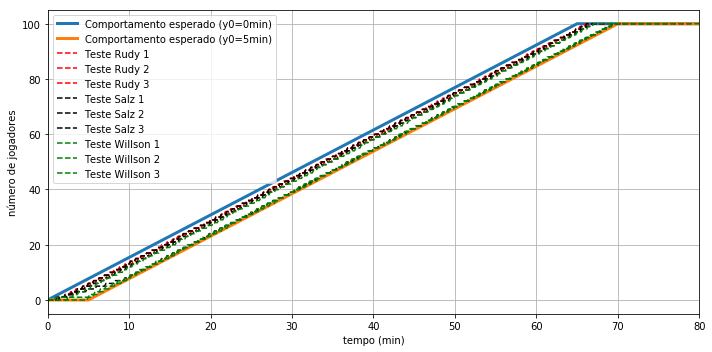
\includegraphics[width=0.8\textwidth]{figuras/network/clientes_script.png}
  \centering

  Fonte: O próprio autor.
\end{figure}

A Figura~\ref{fig:cliente_linear} exibe o crescimento linear de jogadores simultâneos.
%
Tal crescimento está diretamente relacionado ao número de contêineres escalados no aglomerado.
%
Cada jogador realiza as operações descritas na Figura~\ref{fig:movimentacao}.

É notório que o número de jogadores simultâneos é exatamente igual ao número de contêineres na rede de clientes.
%
Dessa forma, garantimos o isolamento entre contêineres, evitando multiplexação de conexões entre processos diferentes.


A partir do comportamento definido na Figura~\ref{fig:cliente_linear}, espera-se que o consumo dos recursos e tempo de resposta corresponda ao seu crescimento, tendendo a uma complexidade linear mínima.
%
Dessa forma, pode-se analisar o comportamento do consumo de recurso, dado o número de jogadores simultâneos.


\section{Considerações Parciais}

Este capítulo descreve a implementação e implantação das arquiteturas, levando em consideração o meio físico na qual foi implantado.
%
Para realizar tal descrição, é necessário citar tecnologias utilizadas e como são conectados.

Durante o desenvolvimento da implantação, é utilizado a linguagem Golang, a qual permitiu o desenvolvimento de forma rápida e eficiente nas aplicações para este trabalho.

Esta escolha implica diretamente nas tecnologias utilizadas.
%
Dessa forma, faz sentido escolher tecnologias que combinem com os objetivos das arquiteturas.

Nesse sentido foram utilizados serviços de armazenamento de dados permanentes e temporários \textit{OpenSource}.
%
Redis e PostgreSQL são os bancos de dados utilizados.
%
Esta escolha é dada pela fácil integração com a linguagem e bibliotecas selecionadas para o desenvolvimento.

Durante o processo de desenvolvimento foi utilizado o processo de integração contínua.
%
Dessa forma, é utilizado o serviço TravisCI para realização de testes e construção de imagens Docker.
%
Por sua vez, o TravisCI utiliza o DockerHub para armazenamento das imagens, as quais são utilizadas para implantar sobre a infraestrutura descrita como ambiente de testes.

Para a execução dos testes, foi utilizado um script para escalar contêineres de forma automática.
%
Dessa forma temos um comportamento linear, podendo utilizar tal comportamento como gráfico, auxiliando na análise.
